\documentclass[journal]{IEEEtran}
\usepackage[a5paper, margin=10mm, onecolumn]{geometry}
\usepackage{amsmath,amssymb,amsfonts,amsthm}
\usepackage{gvv-book}
\usepackage{gvv}
\usepackage{hyperref}

\begin{document}

\title{4.11.23}
\author{Puni Aditya - EE25BTECH11046}
\maketitle

\textbf{Question:}

Find the co-ordinates of the point where the line $\frac{x-3}{-1} = \frac{y+4}{1} = \frac{z+5}{6}$ crosses the plane passing through the points $\brak{\frac{7}{2}, 0, 0}$, $\brak{0, 7, 0}$, and $\brak{0, 0, 7}$.

\textbf{Solution:}

For the intersection of a line
\begin{align*}
    \vec{x} = \vec{p} + \lambda\vec{m}
\end{align*}    
with the plane
\begin{align*}
    \vec{n}^\top\vec{x} = c
\end{align*}
\begin{align}
    \vec{n}^\top\brak{\vec{p}+\lambda\vec{m}} &= c \\
    \vec{n}^\top\vec{p} + \lambda\vec{n}^\top\vec{m} &= c \\
    \lambda &= \frac{c - \vec{n}^\top\vec{p}}{\vec{n}^\top\vec{m}} \label{eq:27} \\
    \vec{x} &= \vec{p} + \brak{\frac{c - \vec{n}^\top\vec{p}}{\vec{n}^\top\vec{m}}}\vec{m} \label{eq:28}
\end{align}

Let the equation of the plane be 
\begin{align}
\myvec{n_1 & n_2 & n_3}\vec{x} = c \label{eq:1}
\end{align}
The three points 
\begin{align*}
    \vec{P_1} = \myvec{\frac{7}{2} \\ 0 \\ 0}, \vec{P_2} = \myvec{0 \\ 7 \\ 0}, \vec{P_3} = \myvec{0 \\ 0 \\ 7}
\end{align*}
satisfy this equation, giving the system:
\begin{align}
    \frac{7}{2}n_1 + 0n_2 + 0n_3 &= c \\
    0n_1 + 7n_2 + 0n_3 &= c \\
    0n_1 + 0n_2 + 7n_3 &= c
\end{align}
This system of equations gives the augmented matrix
\begin{align}
    \myaugvec{3}{
        \frac{7}{2} & 0 & 0 & c \\
        0 & 7 & 0 & c \\
        0 & 0 & 7 & c
    }
    \xleftrightarrow[\text{R}_3 \to \frac{1}{7}\text{R}_3]{\text{R}_1 \to \frac{2}{7}\text{R}_1, \text{R}_2 \to \frac{1}{7}\text{R}_2}
    \myaugvec{3}{
        1 & 0 & 0 & \frac{2c}{7} \\
        0 & 1 & 0 & \frac{c}{7} \\
        0 & 0 & 1 & \frac{c}{7}
    }
\end{align}
From the row-reduced echelon form,
\begin{align}
    n_1 = \frac{2c}{7}, n_2 = \frac{c}{7}, n_3 = \frac{c}{7} \label{eq:2}
\end{align}
Substituting \eqref{eq:2} in \eqref{eq:1},
\begin{align}
    \myvec{\frac{2c}{7} & \frac{c}{7} & \frac{c}{7}}\vec{x} = c
\end{align}
Assuming $c \neq 0$, the equation simplifies to the normal form of the plane, $\vec{n}^\top\vec{x} = c$, which is
\begin{align}
    \myvec{2 & 1 & 1}\vec{x} = 7 \label{eq:plane_eqn}
\end{align}
The vector equation of the line passing through 
\begin{align*}
\vec{p} = \myvec{3 \\ -4 \\ -5}
\end{align*}
with direction vector 
\begin{align*}
    \vec{m} = \myvec{-1 \\ 1 \\ 6}
\end{align*}
is
\begin{align}
    \vec{x} = \myvec{3 \\ -4 \\ -5} + \lambda \myvec{-1 \\ 1 \\ 6} \label{eq:line_eqn}
\end{align}
Using \eqref{eq:28},
\begin{align}
    \vec{x} &= \myvec{3 \\ -4 \\ -5} + \brak{\frac{7 - \myvec{2 & 1 & 1}\myvec{3 \\ -4 \\ -5}}{\myvec{2 & 1 & 1}\myvec{-1 \\ 1 \\ 6}}}\myvec{-1 \\ 1 \\ 6} \\
    \vec{x} &= \myvec{3 \\ -4 \\ -5} + 2\myvec{-1 \\ 1 \\ 6} = \myvec{1 \\ -2 \\ 7}
\end{align}
The co-ordinates of the point of intersection are $\myvec{1 \\ -2 \\ 7}$.

\begin{figure}[h!]
	\centering
	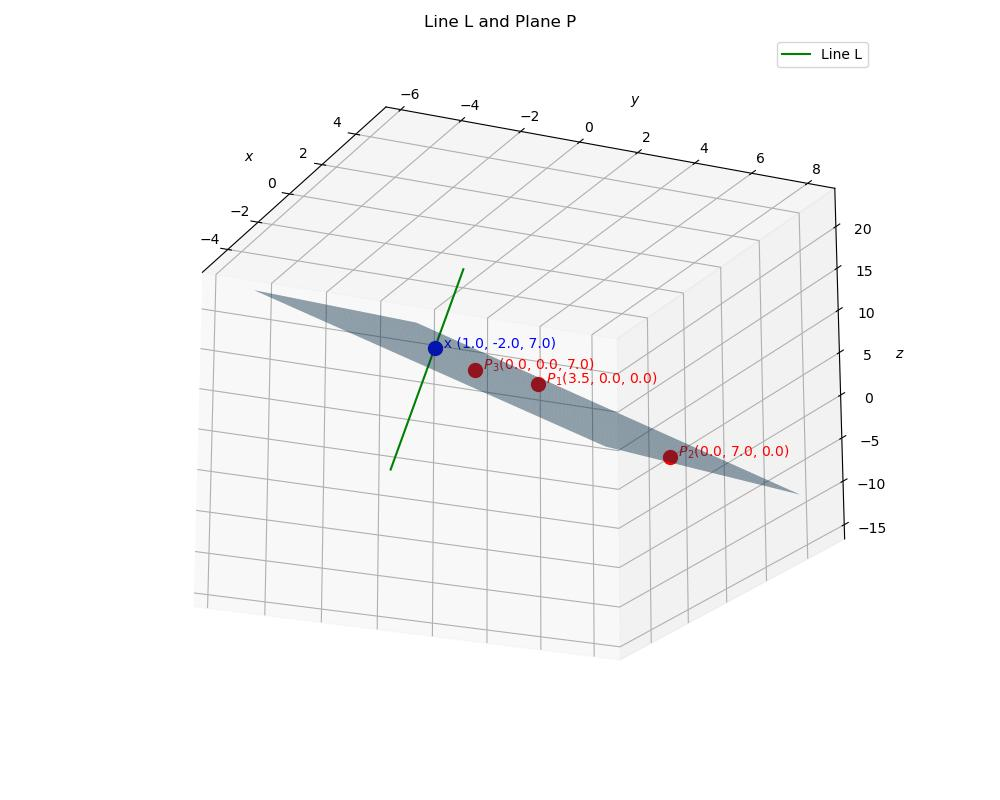
\includegraphics[width=\columnwidth]{figs/plot_c.jpg}
	\caption*{Plot}
	\label{fig:fig}
\end{figure}

\end{document}
